\mysection{\qcd}

Out of the four known interactions given by the current picture of physics, the one that is of the most importance to this work, is the Strong Force\index{Strong Force}. This force is the one responsible for the nuclear stability. It is described by the following lagrangean density\citep{peskin_introduction_1995,halzen_quarks_1984}:

\begin{equation}
\mathcal{L}_{\rm QCD} = -\frac{1}{4}F^{A}_{\alpha\beta}F^{\alpha\beta}_{A}
+\sum_{flavors}
\bar{q}_{A}(i\gamma^{\mu}D_{\mu}-m)_{AB}
q_{B}
\end{equation}

where $F^{\alpha\beta}_{A}$ is the gluon field tensor, $q_{B}$ and $\bar{q}_{A}$ are the fermion fields and $D_{\mu}=\partial_{\mu} + i A_{\mu}/g$ is the covariant derivative. It describes six fermion fields, corresponding to the known fundamental quarks, and also describes their coupling with a non-abelian Yang-Mills field with the \textbf{SU(3)} symmetry. This theory, given its non-abelian nature, has interesting properties that do not appear in electromagnetism.
\par
At first, it is a theory with asymptotic freedom\index{asymptotic freedom}, i.e., the coupling constant\index{coupling constant} decreases as the process under consideration has a larger momentum transfer. This allows one to apply the formalism of perturbation theory\index{perturbation theory} in the calculation of high energy processes. Also, it has non-linear terms in the Yang-Mills sector due to the non-commutative nature of the group. These terms describe the field self-interaction, and also make the theory particularly troublesome to allow calculations. They are also responsible for the decrease of the coupling constant aforementioned. As a result, for low energy processes, the perturbation theory is no longer reliable. Effective models and numerical methods, such as lattice QCD, are then used to try to make predictions. These are classified as non-perturbative methods.
\par
As already mentioned, the coupling constant of the theory varies with energy. The behavior of the coupling constant as one varies the energy of a given process was calculated and is given by\cite{dissertori_quantum_2003}:

\begin{equation}
\alpha_s (q^2) = \frac{2}{b_0 \ln (-q^2/\Lambda^2)}
\end{equation}

The sign of $b_0$ in this equation is opposite to that of QED. As a result, the strength of the interaction grows with distance and is unbounded. The scale $\Lambda$ is a generated scale of QCD and does not depend on quark masses. It is believed that this dynamical scale alone is responsible for the hadron masses, and not the quark masses.

\mysection{\qgp} \label{qgp}

The work by E. Fermi\cite{fermi_high-energy_1950} and L. Landau\cite{lifshitz_statistical_1980,haar_collected_2013} on multiparticle production have paved the way for Hagedorn to develop his bootstrap model\index{model!Hagedorn} in the early sixties. There was already an idea to describe particle physics through the formalism of hydrodynamics. For this to be possible, an understanding of the mass spectrum\index{mass spectrum} of hadrons was necessary. Hagedorn realized that it was possible to find such a spectrum by understanding that heavy hadrons are bound states of lighter hadrons(which are bound states of lighter hadrons(which are bound states of lighter hadrons(...))). With this idea, he developed a formalism that arrived at the following expression for the mass spectrum:

\begin{equation}
\rho(m) \approx c(m_0^2 + m^2)^{k/2} \exp(m/T_0)
\end{equation}

The parameters were meant to be fixed by experiments. The important consequence of this mass spectrum was that the thermodynamical potentials of a hadron gas would have a singularity as $T \rightarrow T_0$. This was the first indication of a possible phase transition.

\par
In the eighties\cite{letessier_hadrons_2002}, with the development of the theoretic understanding of \qcd, it was predicted that, at a certain temperature, the so-called chiral symmetry would be restored. This would then induce a phase transition, bringing about a new state of matter, in which quarks and gluons would be the fundamental degrees of freedom of the partition function. Experimental efforts were put forth to create this new state in the laboratory and, in 2000, CERN announced on a press conference that such a state appeared in its experiments with heavy-ion collisions\citep{letessier_hadrons_2002}.
\par
A few signatures of the \qgp, name assigned to this new state, were found in these experiments\cite{letessier_hadrons_2002}. First, there was the so-called azimuthal anisotropic flow\index{anysotropic flow}. A phenomenon theoretically explained as the conversion of the asymmetry of the geometric distribution of energy in the transverse plane into an asymmetry in momentum space. Besides, there was the strangeness enhancement\index{strangeness} of the observed particles, a hint that a possible chemical equilibrium had been achieved during the collisions. There was also the phenomenon of Jet Quenching, commonly explained by the fact that, unlike in proton collisions, the partons generated in the hard scattering must traverse a dense and hot medium. Its main signature was the suppression of high transverse momentum particles.
\par
The azimuthal anisotropic flow, as previously explained, is related to the asymmetry of the collision. It can be better understood by observing Figure \ref{v2}. In the Figure, it is shown that in the interaction region, in orange, there is a preferential direction for the energy deposition. This geometric property of the distribution is called ellipticity. It is responsible for a larger pressure gradient in the $x$ direction. The gradient is the force responsible for the conversion of the asymmetry from the position space into momentum space. The intensity of this conversion can be calculated through hydrodynamic models. This allows the extraction of properties of the \qgp, such as its viscosity and EOS(Equation of State).

\begin{figure}
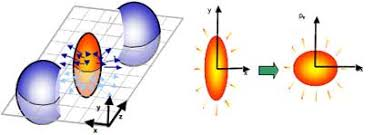
\includegraphics[width=0.5\textwidth]{images/index.jpeg}
\caption[Azimuthal anizotropy representation]{Azimuthal anizotropy representation, picture from \cite{ferrer_exploring_2016}}
\label{v2}
\end{figure}

The strangeness enhancement\index{strangeness!enhancement} is explained through the chemical equilibrium that is achieved in heavy-ion collisions\cite{letessier_hadrons_2002}. This means that the strange particles are generated through thermodynamical processes, not just in the hard-scattering in the early times of the collision. Also, they are not particles that come from the sea quarks inside the colliding nucleons. Normally, this enhancement is measured by a quantity called $ \rm R_{\rm AA} $\index{$ \rm R_{\rm AA} $}, that is defined as the ratio of transverse momentum from pp(proton-proton) to AA(nucleus-nucleus) collisions.
\par
The Jet Quenching phenomena\index{Jet!Quenching} is observed through the $\rm R_{AA}$ taken from the $p_T$ spectrum of particles. This is theoretically interpreted through the parton energy loss while they traverse the plasma, as illustrated in Figure \ref{arrefecimento}. Beyond the spectrum suppression, jet analysis has also revealed that there are distinct fragmentation patterns, as opposed to the vacuum case, hinting a parton-medium interaction\cite{denterria_jet_2009}.

\begin{figure}
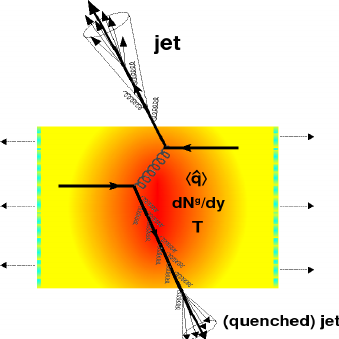
\includegraphics[width=0.5\textwidth]{images/quenching.png}
\caption[Schematics of a parton traversing the medium.]{Schematics of a parton traversing the medium. Figure from \cite{denterria_jet_2009}}
\label{arrefecimento}
\end{figure}

The description of the medium that JEWEL (Jet Evolution With Energy Loss) uses, in its default settings, consists of calculating the partition function by assuming an ideal quantum free gas of non-interacting particles. This model is based on the idea of asymptotic freedom\index{asymptotic freedom}, which is the decrease of the interaction of the partons with the increase of temperature.
\par
This model is necessary to translate temperature profiles into a scattering center density. This is done though the following equation\cite{bjorken_highly_1983,zapp_jet_2006}:

\begin{equation}
n_s= 2 g_g \zeta(3) \frac{T^3}{2 \pi^2}
\end{equation}

Results calculated with the lattice \qcd approach corroborate that this expressions are valid for $T = 200 \, \rm MeV$\cite{letessier_hadrons_2002}. Before that, at $T \approx 185 \, \rm MeV$, there is a rapid transition from this fluid to the free hadron gas\index{critical temperature}. These equations for an ideal relativistic quantum gas are used in some Jet Quenching models\footnote{such as JEWEL(Jet Evolution With Energy Loss)} for the description of the medium.

\mysubsection{Hydrodynamics of the \qgp}

Hydrodynamics is the formalism chosen to model the evolution from thermalization until the free streaming of particles. The conversion of hydrodynamic calculations into free hadrons is made with the Cooper-Frye prescription\index{prescription!Cooper-Frye}. Hydrodynamics is essentially approached through the relativistic energy-momentum tensor\cite{florkowski_phenomenology_2010}

\begin{equation}
T^{\mu \nu} = \epsilon u^{\mu} u^{\nu} + P \Delta^{\mu \nu}
\label{tensor}
\end{equation}

Where $\Delta^{\mu \nu} = g^{\mu \nu} - u^\mu u^\nu$ is the projection operator orthogonal to $u^\nu$, $P$ is the local pressure and $\epsilon$ is the energy density. The conservation equation\index{conservation equation} for this tensor is:

\begin{equation}
\partial_{\mu} T^{\mu \nu} = 0
\label{conservation_eq}
\end{equation}

This equation has, in total, six independent quantities, four from the local velocity plus two from energy density and pressure. There are four equations from energy-momentum conservation, which leaves two unknowns. The normalization of the four-velocity plus the equation of state then solve the system.
\par
When the system is out of equilibrium, the energy-momentum tensor is different from the one in equation \eqref{tensor}. In the first order, it assumes the form:

\begin{equation}
T^{\mu \nu} = \epsilon u^{\mu} u^{\nu} + P \Delta^{\mu \nu} + \tau^{\mu \nu}
\end{equation}

Where $\tau^{\mu \nu}$ corresponds to a deviation from equilibrium state. This form is constructed by creating an artificial equilibrium state by considering the local energy density, which is a well-defined quantity\cite{romatschke_new_2010}. Here $\tau^{\mu \nu}$ is required to be symmetric due to the conservation of angular momentum.
\par
At this point, it is useful to define the projection operator:

\begin{equation}
\Delta^{\alpha \beta}_{\mu \nu} = \frac{1}{2} \left[ \Delta^{\alpha}_{\mu}\Delta^{\beta}_{\nu} + \Delta^{\alpha}_{\nu}\Delta^{\beta}_{\mu} - \frac{2}{3} \Delta^{\alpha \beta}\Delta_{\mu \nu} \right]
\label{projection}
\end{equation}

It is symmetric in $\alpha$ and $\beta$ and in $\mu$ and $\nu$, and the resulting projection is traceless. This operator helps us to decompose $\tau^{\mu \nu}$ in three different components with simple physical interpretations. The code to integrate numerically these equations will have to be provided with differential equations for the extra degrees of freedom included by $\tau^{\mu \nu}$. This part is usually chosen according to a specific model.
\par 
Besides the conservation equation \eqref{conservation_eq}, there might be other currents (Such as baryon number, strangeness number, etc) that satisfy a conservation equation as well:

\begin{equation}
\partial_{\mu} j^{\mu} = 0
\end{equation}

Each current included also comes with a conservation equation, so the system is still solvable.

\mysection{Relativistic Heavy-Ion Collisions}

The experimental method used to study the QGP is the collision of heavy nuclei at relativistic velocities. The general picture for such a collision can be seen in Figure \ref{heavy_ion}. Two Lorentz contracted nuclei approach each other at relativistic speed and then collide, leaving energy in the interaction region. The matter deposited in the interaction region then thermalizes in about $\sim 1 {\rm fm/c}$. This stage is currently the most poorly understood and the source of the largest uncertainty. After thermalization, the hot system expands until $\sim 10 {\rm fm/c}$, a stage that can be simulated with hydrodynamics codes using as input the models that attempt to describe the initial energy density profile. During the hydro evolution, the system reaches the hadronization stage. After the hadron stage the kinetic freeze-out happens in which particles start to stream freely until they reach the detectors at about $\sim 10^{15} {\rm fm/c}$.

\begin{figure}
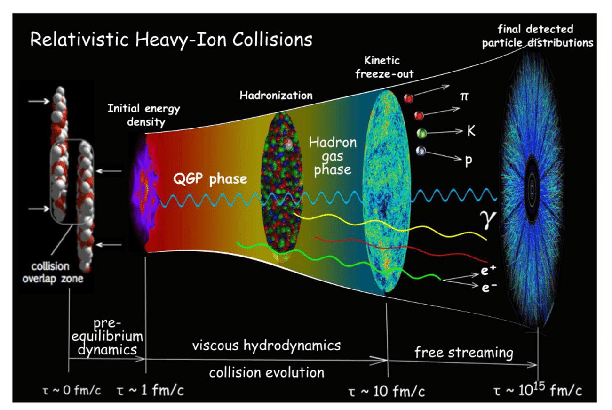
\includegraphics[width=1.0\textwidth]{images/Illustration-of-the-dynamical-evolution-of-relativistic-heavy-ion-collisions-and-the-QGP.png}
\caption[Heavy-ion collision scheme]{Heavy-ion collision scheme, picture from \cite{scharenberg_hot_2018}}
\label{heavy_ion}
\end{figure}

\mysubsection{Initial Conditions} \label{IC}

For the initial conditions, as explained, models are used to predict the energy density profiles that result from the early dynamics of the collision. One of the first models used was Glauber wounded nucleon model\cite{miller_glauber_2007}. Later, models that implemented sophisticated ideas inspired by QCD were developed. Here we studied three different models. First, we used JEWEL\cite{zapp_monte_2009,zapp_local_2011} default model, which is a Glauber like without any type of fluctuation in the nucleons positions. Then, we used \trento\cite{moreland_alternative_2015}, which is also Glauber inspired, but parametric in nature, and can be tuned to fit certain experimental results and extract qualitative behavior of the initial conditions. And then we used MC-KLN\cite{drescher_effects_2007}, based on the color-glass condensate formalism.


\begin{figure}
\subfloat[Glauber]{
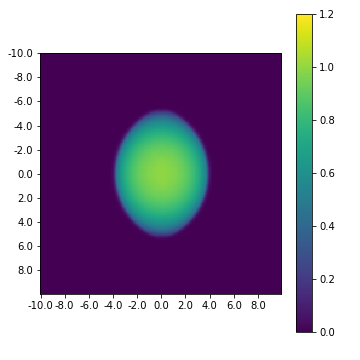
\includegraphics[width=0.3\textwidth]{images/glauber.png}\label{ic_glauber}
}
\label{glauber}
\subfloat[MC-KLN]{
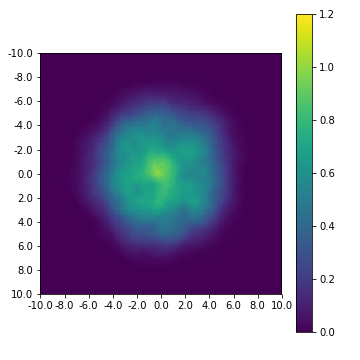
\includegraphics[width=0.3\textwidth]{images/mc_kln.png}\label{ic_kln}
}
\subfloat[\trento]{
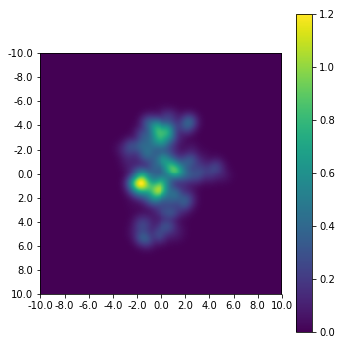
\includegraphics[width=0.3\textwidth]{images/trento.png}\label{ic_trento}
}
\caption{Energy density in arbitrary units for different initial condition models. The energy density is displayed in arbitrary units.}
\label{ic}
\end{figure}

\mysubsection{Glauber smooth model} \label{glauber}

The implementation of the background medium used by JEWEL is an idealized and smooth Glauber model. For nuclei density, a Wood-Saxon distribution is assumed:

\begin{equation}
\rho({\overrightarrow{\bf \it r}}) = \frac{1}{1+\exp(\frac{r-R}{a})}
\end{equation}

Where $R$ is the nuclei radius and $a$ represents a \emph{skin-depth} of the nuclei. This profile density if almost entirely constant for $r<R$. The transverse density is taken from the longitudinal integration:

\begin{equation}
T_A(x,y) = \int dz \, \frac{1}{1+\exp(\frac{r(x,y,z)-R}{a})}
\end{equation}

This $T_A$ is called the thickness function. The combination of the thickness function of both nuclei then determines the energy density:


\begin{equation}
\begin{split}
\epsilon (x,y) &\propto T_A(x-\frac{b}{2},y) \left[ 1 - \exp \left( - \sigma_{NN} T_B(x+\frac{b}{2},y) \right) \right] \\ & + T_B(x+\frac{b}{2},y) \left[ 1 - \exp \left( - \sigma_{NN} T_A(x-\frac{b}{2},y) \right) \right]
\end{split}
\end{equation}

Where $\sigma_{NN}$ is the nucleon-nucleon cross-section. An example of this energy profile can be observed in Figure \ref{ic}(a). The name smooth used here references the lack of \emph{lumpiness} in this profile, as compared to the others in Figure \ref{ic}.

\mysubsection{T$_{\rm R}$ENTo} \label{trento}

T$_{\rm R}$ENTo\cite{moreland_alternative_2015} is a model for initial conditions for heavy-ion collisions based on the Glauber model. It is based on the idea of the thickness function:

\begin{equation}
T_A (x,y) = \int {\rm d}z \, \rho^{\rm part} (x,y,z)
\end{equation}

Which is built from the density of participants $\rho^{\rm part} (x,y,z)$. Once the thickness functions of both nuclei are defined, a scalar function is defined as:

\begin{equation}
f = \left( \frac{T^p_A+T^p_B}{2} \right)^{1/p}
\end{equation}

Where $p$ is a free parameter. This is a generalized mean and is taken to be proportional to the entropy deposition. This function has a general behavior that changes continuously with the parameter $p$, interpolating between maximum and minimum. Each value corresponds to a qualitatively different entropy deposit mechanism. The qualitative behavior of this function can be seen in Figure \ref{trento_thick}.

\begin{figure}
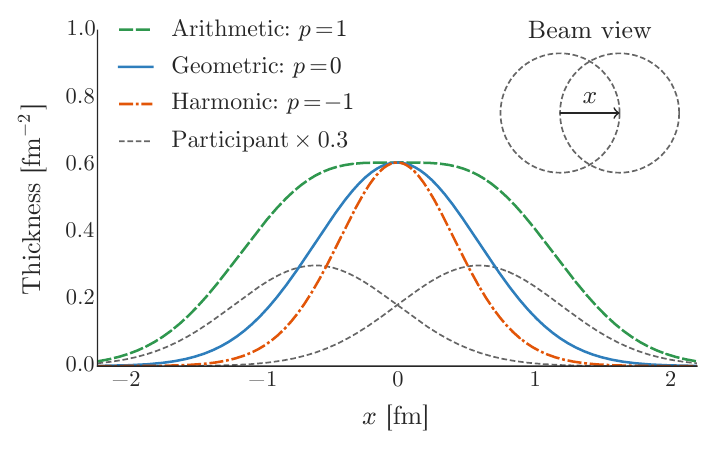
\includegraphics[width=1.0\textwidth]{images/trento_thick.png}
\caption[$T_RENTo$ reduction thickness.]{$T_RENTo$ reduction thickness. The dashed lines correspond to nucleon profiles and the colored lines correspond to the reduced thickness for different values of $p$. Picture from \cite{moreland_alternative_2015}}
\label{trento_thick}
\end{figure}

The participant densities are built by considering pairs of nucleons, one from each nucleus. Their positions are sampled from a Woods-Saxon potential. Then for each pair the probability of collision is taken as:

\begin{equation}
P_{coll} = 1 - \exp \left[ -\sigma_{gg} \int dx \, dy \int dz \, \rho_A \int dz \, \rho_B \right]
\end{equation}

Here we have that $\sigma_{gg}$ is adjusted so that the total proton cross-section is $\sigma_{NN}$\cite{moreland_alternative_2015}. If the nucleons do collide, then the thickness function is built from the sum of each nucleon density, which is taken to be a gaussian. So each nucleon contributes with a thickness function given by:

\begin{equation}
T_{N} = w \int dz \, \rho_N (x,y,z) 
\end{equation}

Where $w$ is a random weight sampled from a gamma distribution with unity mean:

\begin{equation}
P_k(w)=\frac{k^k}{\Gamma(k)} w^{k-1} e^{-kw}
\end{equation}

This creates an extra degree of fluctuation that will be encoded in a parameter $k$ that can be chosen to fit experimental results. An example of a $\rm T_RENTo$ profile for $p=0$, which is a tune that reproduces IP-Glasma behavior, can be seen in Figure \ref{ic}(c). The effects of fluctuations can be observed in the figure.

\mysubsection{MC-KLN} \label{mckln}

The MC-KLN\cite{drescher_effects_2007} model is based on the color glass condensate approach. The key idea is that a nuclei is essentially a gluon wall with a wavelength bigger than the contracted longitudinal size of the other nuclei. So the collision occurs in a coherent manner. A saturation scale can be defined such that below it the occupation number of gluons is constant, and above, we have a distribution that obeys the BFKL equations\cite{kovchegov_quantum_2012}. The saturation scale is defined in terms of the thickness function, according to:

\begin{equation}
Q_{s,A}^{2} (x, \textbf{r}_{\perp}) = 2 \, {\rm Gev}^2 \left( \frac{T_A (\textbf{r}_{\perp}) / p_A(\textbf{r}_{\perp}) }{1.53} \right) \left( \frac{0.01}{x} \right)^{\lambda}
\end{equation}

Where $T_A (\textbf{r}_{\perp})$ is the thickness function and $x$ is the fraction of the momentum carried by the gluon in the distribution. $p_A({\mathbf{r}_{\perp}})$ is the probability of finding at least nucleon at a given transverse coordinate. In this way, the model proceeds by randomly picking nucleon positions according to a Woods-Saxon potential, and then it determines the thickness function, finally determining the saturation scales. The gluon distributions are then combined through:

\begin{equation}
\frac{dN_g}{dyd^2\textbf{r}_{\perp}} \sim \int \frac{d^2p_{\perp}}{p^2_{\perp}} \int d^2 k_{\perp} \phi (n_{part,A}) \phi (n_{part,B})
\end{equation}

where:

\begin{equation}
\phi(x,k_{\perp}\;\textbf{r}_{\perp}) \sim \frac{1}{\alpha(Q_s^2)} \frac{Q_s^2}{\max (Q_s^2,k_{\perp}^2)}
\label{gdf_kln}
\end{equation}

And $\phi$ is the gluon distribution function. An example of an MC-KLN generated profile can be seen in Figure \ref{ic}(b). The larger spread of the energy density is a consequence of the tail of the gluon distribution in Equation \eqref{gdf_kln}.

\mysection{Hydrodynamics} \label{hydro}

The implementation of the hydrodynamics involves developing a numerical method for integration of the hydrodynamic equations, as well as an Equation of State and the differential equations satisfied by the independent components of the $\tau^{\mu \nu}$ tensor. Here we used two ways to model this stage of the collision. First, as the JEWEL default, we use the Bjorken longitudinal expansion model, which is only an approximation. For a more realistic treatment, we used the 2+1 code v-USPhydro.

\mysubsection{Bjorken expansion} \label{bjorken}

One of the first models developed to calculate the evolution of the QGP was the one developed by Bjorken that approximates the system to a one-dimensional system and considers the expansion only in the longitudinal direction. This model then predicts a decay of the energy density that can explain the plateau in the rapidity spectrum. The idea is that we have a blast wave in the longitudinal direction that is bound by the speed of sound in the medium:

\begin{equation}
T = T_0 \left( \frac{\tau_0}{\tau} \right)^{v_s^2}
\end{equation}

where $\tau_0$ and $T_0$ are chosen to fit experimental data, mainly the $\frac{dN}{d\eta}$ observable. Since the speed of sound is calculated, for a relativistic ideal quantum gas, to be $v_s^2=\frac{1}{3}$, we have a complete description of the temperature evolution of the system. The values chosen in JEWEL\cite{zapp_perturbative_2013} are $\tau_0=0.5 \, {\rm fm/c}$ and $T_0=530 \, {\rm MeV}$.

\mysubsection{v-USPhydro} \label{vusp}

The hydrodynamics model used here is v-USPhydro\cite{noronha-hostler_bulk_2014,noronha-hostler_bulk_2013,noauthor_jacquelyn_nodate}. It utilizes the Lagrangian method to implement the integration of the conservation equations that describes the hydrodynamics. This method consists, as an alternative to the grid methods, of discretizing the fluid density profile into particles and allowing their positions to evolve as well. One of the advantages of this approach is that it can be efficiently applied to unbound systems, as is the case of nuclei collisions. This formalism is called Smoothed Particle Hydrodynamics.
\par
The idea is to use a finite number of cells to describe the fluid. One then defines a normalized kernel:

\begin{equation}
\int W [\mathbf{\rm r};h]d^2 \mathbf{\rm r} = 1
\end{equation}

where $\textbf{\rm r}$ is a transverse position coordinate and $h$ is a parameter that plays a similar role to the grid spacing in the Euler method. This kernel can then use the cells to calculate the value of a field at any point in space:

\begin{equation}
\tau \gamma \sigma \rightarrow \sigma^* (\mathbf{\rm r}, \tau) = \sum_{\alpha=1}^{N_{SPH}} \nu_\alpha W [ \mathbf{\rm r} - \mathbf{\rm r}_\alpha(\tau);h]
\end{equation}

Where $\tau$ is the proper time, $\gamma$ is the relativistic factor. $\sigma$ is the entropy density and $N_{SPH}$ is the number of Smoothed Particle cells. The conservation of $\tau \gamma \sigma$ is then equivalent to:

\begin{equation}
\sum_{\alpha=1}^{N_{SPH}} \nu_\alpha = K
\end{equation}

where $K$ is a constant and the $\nu_\alpha$ are chosen to match an initial distribution. The entities that occupy the positions $\boldsymbol{\rm r}_{\alpha}$ are referred to as SPH particles. Now, given some extensive quantity associated to the density $a(\boldsymbol{\rm r},\tau)$, the discretized version of it will be:

\begin{equation}
a(\boldsymbol{\rm r},\tau) = \sum_{\alpha=1}^{N_{SPH}} \nu_{\alpha} \frac{a(\boldsymbol{\rm r}_{\alpha} (\tau))}{\sigma^*(\boldsymbol{\rm r}_{\alpha} (\tau))} W [ \boldsymbol{\rm r} - \boldsymbol{\rm r}_\alpha(\tau);h]
\end{equation}

And the derivative of it will be:

\begin{equation}
\frac{d}{d\boldsymbol{\rm r}} a(\mathbf{\rm r},\tau) = \sum_{\alpha=1}^{N_{SPH}} \nu_{\alpha} \frac{a(\boldsymbol{\rm r}_\alpha (\tau))}{\sigma^*(\boldsymbol{\rm r}_\alpha (\tau))} \frac{d}{d\boldsymbol{\rm r}} W [ \boldsymbol{\rm r} - \boldsymbol{\rm r}_\alpha(\tau);h]
\end{equation}

So, a knowledge of the derivative of the kernel function allows one to calculate the derivative of any extensive quantity. Similarly, the proper-time derivative:

\begin{equation}
\frac{d}{d \tau} a(\mathbf{\rm r},\tau) = \sum_{\alpha=1}^{N_{SPH}} \nu_{\alpha} \frac{a(\boldsymbol{\rm r}_\alpha (\tau))}{\sigma^*(\boldsymbol{\rm r}_\alpha (\tau))} \frac{d\boldsymbol{\rm r}_\alpha (\tau)}{d \tau} \frac{d}{d\boldsymbol{\rm r}_\alpha (\tau)} W [ \boldsymbol{\rm r} - \boldsymbol{\rm r}_\alpha(\tau);h]
\end{equation}

The equations of motion for the fluid are\cite{denicol_effect_2009,denicol_effect_2010}:

\begin{equation}
\gamma \frac{d}{d\tau} \left[ \frac{(\epsilon + p + \Pi)}{\sigma} u^{\mu} \right] = \frac{1}{\sigma} \partial^{\mu} (p+\Pi)
\end{equation}

\begin{equation}
\gamma \frac{d}{d \tau} \left( \frac{s}{\sigma} \right) + \left( \frac{\Pi}{\sigma} \right) \frac{\theta}{T} = 0
\end{equation}

\begin{equation}
\tau_{\Pi} \gamma \frac{d}{d\tau}\left( \frac{\Pi}{\sigma} \right) + \frac{\Pi}{\sigma} + \left( \frac{\zeta}{\sigma} \right) \theta = 0
\end{equation}

where $\Pi$ and $\zeta$ are the bulk and shear viscosity, $\epsilon$, $s$ and $\sigma$ are the energy density, the entropy density, and the system density, respectively. $T$ is the temperature and $\theta$ is the four divergence of the velocity that describes the expansion rate of the system. v-USPhydro integrates these equations using the discretization procedure described above using a Runge-Kutta method and then calculates freeze-out surface and temperature profile and other quantities. For this work, we are interested in the temperature profile.

\mysection{Jet Quenching}

\mysubsection{Jet Evolution With Energy Loss (JEWEL)}

JEWEL\cite{zapp_jewel_2014, zapp_monte_2009, zapp_perturbative_2013} is a Monte-Carlo implementation of a perturbative formalism, called the BDMPS-Zakharov formalism which treats elastic collisions and radiation for a parton moving in a dense environment. One of the issues that appears when one wants to consider Monte-Carlo implementations of quantum phenomena is that one must deal with amplitudes, not probabilities. So JEWEL addresses this by the definition of a parameter that will separate the cases where interference might occur. This parameter is called the gluon formation time:

\begin{equation}
\tau = \frac{\mathbf{k}^2}{2\omega}
\end{equation}

Where $\mathbf{k}$ is the radiation momentum, and $\omega$ is the radiation energy. This parameter is used to determine if two successive scatterings are within the formation time of an emission. If that is the case, JEWEL treats the scattering centers as coherent sources of the \emph{gluonstrahlung}.
\par
The algorithm implemented in JEWEL is the following. First, a pair of partons is generated through hard scattering in a point in transverse space proportional to the energy-density. Then these partons are propagated through the medium. In this process they will lose energy through collisions and through parton-shower. After they escape the medium, the event is given to PYTHIA\cite{sjostrand_pythia_2006} to perform fragmentation and hadronization.
\par
The parton shower is implemented in JEWEL through the virtuality ordering procedures that resums leading logarithm of pQCD. Is is implemented through the so-called Sudakov form factor:

\begin{equation}
\mathcal{S}(t_h,t_c) = \exp \left\{ -\int_{t_c}^{t_h} \frac{{\rm d} t}{t} \int_{z_{\rm min}}^{z_{\rm max}} {\rm d} z \sum_b \frac{\alpha_s (k_{\bot}^2)}{2\pi} \hat{P}_{ba} (z) \right\}
\end{equation}

This can be interpreted as the probability that a parton emits no radiation between the scales $t_h$ and $t_c$. The function $\hat{P}(z)$ is the so-called Altarelli-Parisi splitting functions. This Sudakov form-factor is used to determine the scale of the next splitting in the parton shower. This shower will behave as if it was in vaccum. It is the collisional process that allows for the generation of further virtuality evolution and will be responsible for medium-modifications of the jet.
\par
The collisional part of JEWEL is treated through simple $2 \rightarrow 2$ matrix elements squared. A thermal mass is attributed to the gluons representing the scattering centers. This is the Debye mass given by $\mu_D \approx 3T$. The $2 \rightarrow 2$ cross-section then takes the form:

\begin{equation}
\sigma_i (E,T) = \int {\rm d}|\hat{t}| \int {\rm d}x \sum_{j \in \{ q,\overline{q},g \}} f_{j}^{i} (x,\hat{t}) \frac{{\rm d}\hat{\sigma}_j}{{\rm d} \hat{t}} (x\hat{s}, |\hat{t}|)
\end{equation}

Where $\hat{s}$ is the collision energy on the center of mass, $\hat{\sigma}$ is the $2 \rightarrow 2$ scattering cross-section. And $f_j^i(x,\hat{t})$ is the PDF that describes the probability of finding a parton $j$ in a parton $i$ with momentum fraction $x$ at the momentum transfer $\hat{t}$. The PDF shown in the above equation represents the initial-state radiation emitted by the projectile that allows the calculation to approximate higher-order terms in the perturbative calculation. In this prescription, Bremsstrahlung is automatically taken into account.
\par
The main difficulty in implementing Monte-Carlo simulations for quantum systems is the fact that quantum systems are not Markov chains. There is always the presence of interference effects that must be taken into account. JEWEL does it so using a parametrically formation time attributed to the radiated gluons from the projectile. If the formation time of emission is longer than two consecutive scatterings, then these cases must be analyzed and dealt with specially. 
\par
To summarize, the steps taken by JEWEL are the following:

\begin{itemize}
\item[1] First, a hard scattering is generated in PYTHIA, producing the partons to be propagated;
\item[2]JEWEL evolves this parton state with collisions and radiation, taking into account the non-abelian LPM effect;
\item[3]Once the partons are close enough to mass shell and have escaped the medium, the final partonic state is handed back to PYTHIA;
\item[4]PYTHIA performs the fragmentation of the partonic final state and hadronization, as well as the resonance decays;
\end{itemize}


\mysection{Hadronization}

Jets, as described before, are a natural consequence of confinement. The formation of jets from partons is called hadronization. Unfortunately, hadronization is a low energy process and falls within the realm of non-perturbative Quantum Chromodynamics. As an implication, a lot of models are used to describe this process and not first principle calculations. One such model is the Lund model. This is the model implements by PYTHIA, which was used to convert the final partonic state provided by JEWEL into a set of hadrons.

\mysubsection{Lund Model}

The Lund string model is based on the idea of tunneling in quantum mechanics. The equation that must be satisfied by the wavefunction of a quark coming out of the Dirac sea is\cite{wong_introduction_1994}:

\begin{equation}
\left[ (p-A)^2 -m^2 \right] \psi = 0
\end{equation}

Where $p$ is the particle 4-momentum, $A$ is the four potential and $m$ is the particle mass.The potential between a quark and an antiquark is linear in the $z$ coordinate. Expanding this equation and separating the variables, we can arrive at:

\begin{equation}
\psi = \exp [ i(p_x x + p_y y -Et) ] f(z) = 0
\end{equation}

Where $f(x)$ satisfies the equation:

\begin{equation}
\left\{ [E - A_0(z)]^2 - p_z^2 - m_T^2 \right\} f(z) = 0
\end{equation}

Where $m_T=\sqrt{p_T^2 + m^2}$. Here we have assumed only a scalar potential $A_0$\cite{wong_introduction_1994}. Dividing this equation by $m_T$ we arrive at:

\begin{equation}
\left[ \frac{p_z^2}{2m_T} + V_{eff}(z) - E_{eff} \right] f(z) = 0
\end{equation}

Which is a Schrödinger equation for an effective energy $E_{eff}=0$ and an effective potential of the form:

\begin{equation}
V_{eff}(z) = \frac{m_T}{2} - \frac{[ E-A_0(z) ]^2}{2 m_T}
\end{equation}

\begin{figure}
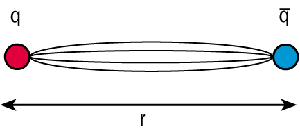
\includegraphics[width=0.5\textwidth]{images/lund.png}
\caption{Schematics of a quark and an antiquark and the field between them.}
\label{lund_scheme}
\end{figure}

We assume the potential to be linear. To see why this is the case, one can look at Figure \ref{lund_scheme}. The lines of force do not spread into space. This happens because the gluon field carries charge and it is attracted to itself. The gluon field also satisfies Gauss's law. As a result, the flow in any cross-sectional surface between the quarks must be the same. This implies a constant electric field, which in turn, implies a linear potential:

\begin{equation}
A_0(z) = -\kappa z
\end{equation}

Coupling this formalism with the WKB method, we arrive at\cite{wong_introduction_1994}:

\begin{equation}
P = \exp \left\{ - \frac{\pi m_T^2}{\kappa} \right\}
\end{equation}

This equation indicates that particles with a greater transverse mass have a lower probability of being produced and explains the hadrochemistry observed in jets. The mechanism just explained is the Schwinger particle production mechanism. It was created to describe pair creation in strong electric fields in QED. It was adapted to the context of QCD where it could describe the behavior of jets, e.g. their multiplicity.
\par
Once the parton pairs no longer have enough energy to break the strings, they become resonances that decay into hadrons in a Lorentz invariant way. At this stage, phase space considerations are used to determine the momenta of the decay products\cite{sjostrand_pythia_2006}.